\documentclass[a4paper,11pt]{article}
\usepackage[T1]{fontenc}      % codifica dei font
\usepackage[utf8]{inputenc}
\usepackage[italian]{babel}
\usepackage{lipsum}
\usepackage{comment}
\usepackage{url}
\usepackage{amsfonts}
\usepackage{graphicx}
\begin{document}
% lettere accentate da tastiera
% lingua del documento
% genera testo fittizio
% per scrivere gli indirizzi Internet
\author{Linpeng Zhang}
\title{Tutorato AFL}
\maketitle
\begin{abstract}
    Per errori/dubbi/problemi: linpeng.zhang@studenti.unipd.it.% \\Note:
\end{abstract}
\tableofcontents
\section{Lez7}
\subsection{Esercizi}
\begin{enumerate}
    \item Sia $L=\{0^{2n}10^n \ |\  n\in\mathbb{N}\}$. Dire se il linguaggio è regolare e, a seconda della risposta (da motivare), definire una CFG o un automa che accetti $L$;
    \item Costruire un automa a pila che accetti $L=\{a^nb^n \ |\  n\geq 1\}$;
    \item Definire una CFG che riconosce $L=\{a^nb^n \ |\  n\geq 1\}$;
    \item Dato il linguaggio: $L=\{w\in\{a,b,c\}^* \ | \ \#a(x)+\#b(x)=\#c(x)\}$
    \\dire se L è regolare, dare una CFG o un'espressione regolare, costruire un automa.
    \item Definire un automa che accetta stringhe in $\{a, b\}^*$ che non sono nella forma $ww$.
\end{enumerate}
\subsection{Soluzioni}
\begin{enumerate}
    \item si può dimostrare con il PL che $L$ non è regolare, prendendo ad esempio $w=0^{2h}10^h$. Una CFG che genera $L$ è data da:\\ $S\rightarrow 1|00S0$;
    \item Un automa a pila che accetta tale linguaggio è:\\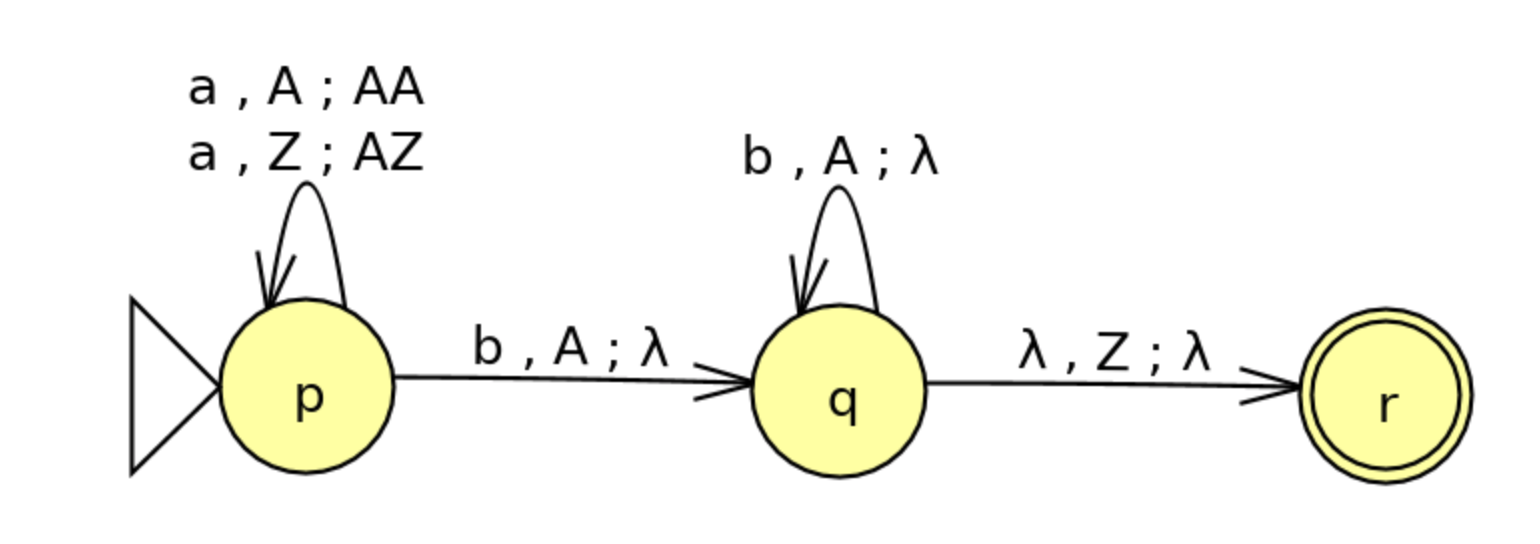
\includegraphics[scale=0.4]{Lez7sol2.png}
    \item una CFG è:\\
    \begin{minipage}{\linewidth}
       \centering $S \rightarrow aSb\ |\ ab$
   \end{minipage}
   \item il linguaggio non è regolare. Una CFG è:\\
   \begin{minipage}{\linewidth}
      \centering $S \rightarrow SaScS\ |\ SbScS\ |\ ScSaS\ |\ ScSbS \ | \ \epsilon$
   \end{minipage}
   Un automa a pila si costruisce inserendo le transazioni in modo che:
   \begin{itemize}
    \item se leggo $a$ o $b$ e ho $Z_0$ o $X$ in cima inserisco una $X$;
    \item se leggo $c$ e ho $Z_0$ o $Y$ in cima inserisco una $Y$;
    \item se leggo $a$ o $b$ e ho $Y$ in cima consumo una $Y$;
    \item se leggo $c$ e ho $X$ in cima consumo una $X$;
   \end{itemize}
   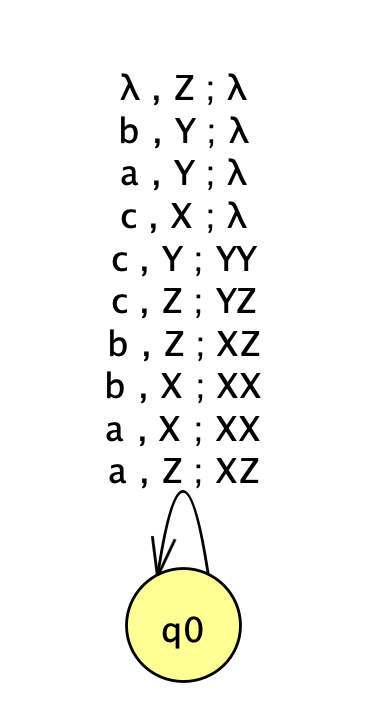
\includegraphics[scale=0.5]{Lez7sol4.png}
    \item Una stringa non è nella forma $ww$ se ha almeno una coppia di simboli a distanza $|w|$ diversi tra di loro. Quindi, un automa a pila che riconosce tale linguaggio deve leggere K caratteri, finché ad un certo punto, nondeterministicamente, pensa di aver trovato un simbolo che sarà diverso a distanza $|w|$. Successivamente ne legge altri K, svuotando la pila. Poi ne legge un numero arbitrario (ad esempio L), legge il carattere diverso ed infine legge altri L caratteri, svuotando la pila. Infine svuota anche $Z_0$.\\ Da questa intuizione segue l'automa seguente:\\ 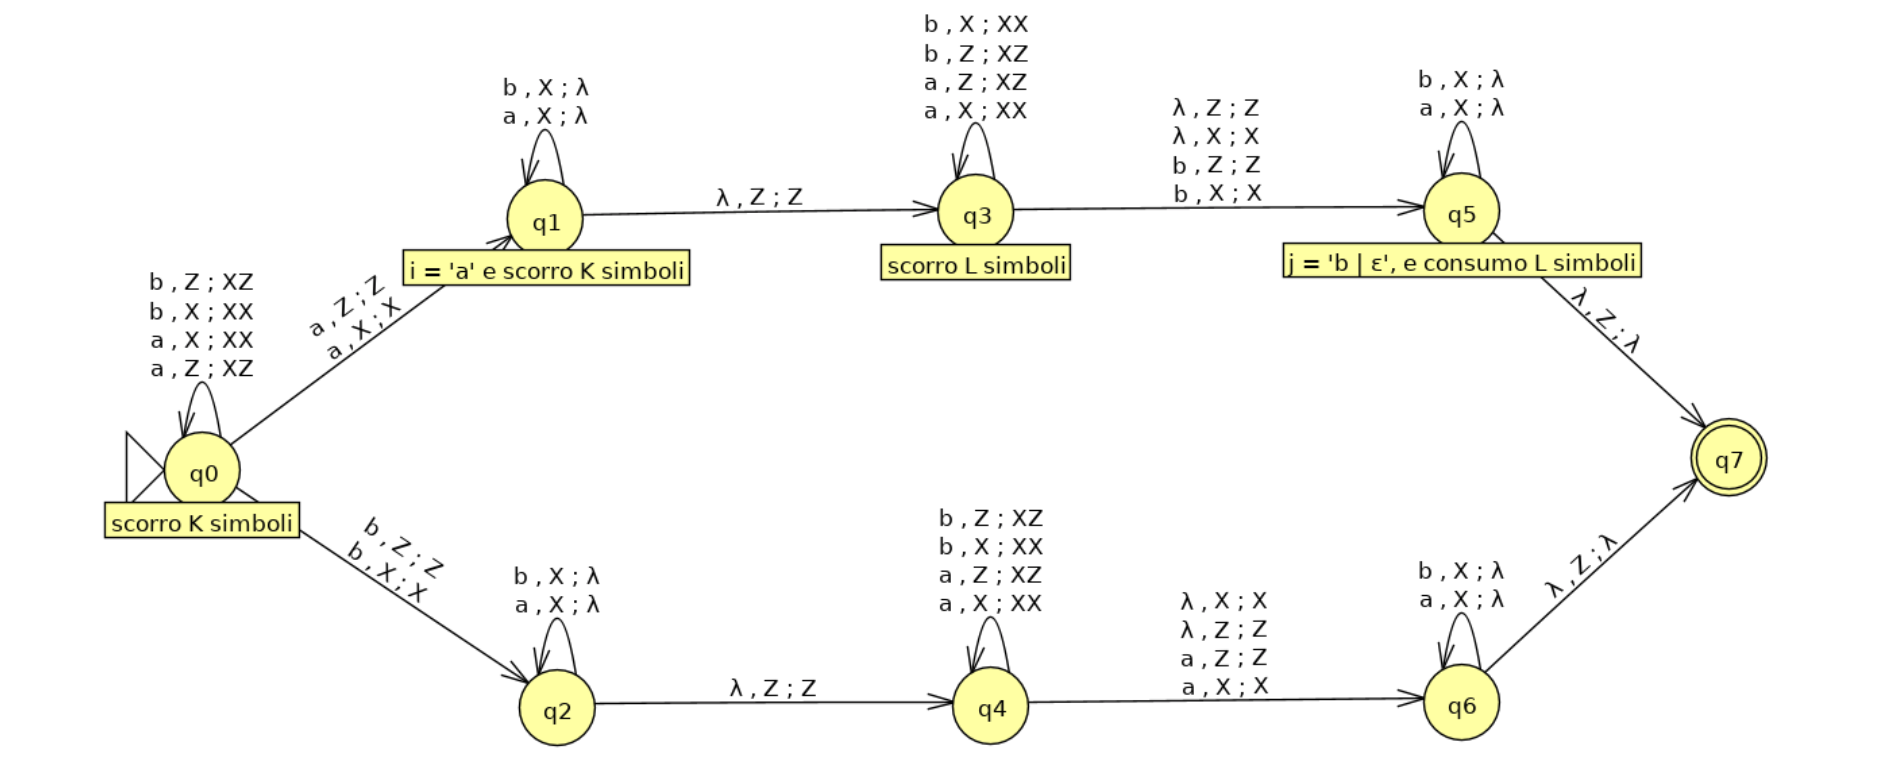
\includegraphics[scale=0.5]{Lez7sol5.png}
       %   \item si può dimostrare che A genera $L_A=\{a^nb^m|n=m+1$ oppure $n=m$ con $n>0,m\geq 0\}$, B genera $L_B=\{a^nb^m|m=n+1$ oppure $n=m$ con $m>0,n\geq 0\}$. Dalle due asserzioni precedenti si dimostra che S genera $L_S=\{a^nb^m|n=m+1$ oppure $n=m$ con $n,m>0\}$: infatti S produce le stringhe che produce B con una a all'inizio, e la correttezza segue dalla definizione.\\
   %  Un automa a pila che accetta tale linguaggio è:\\
  %  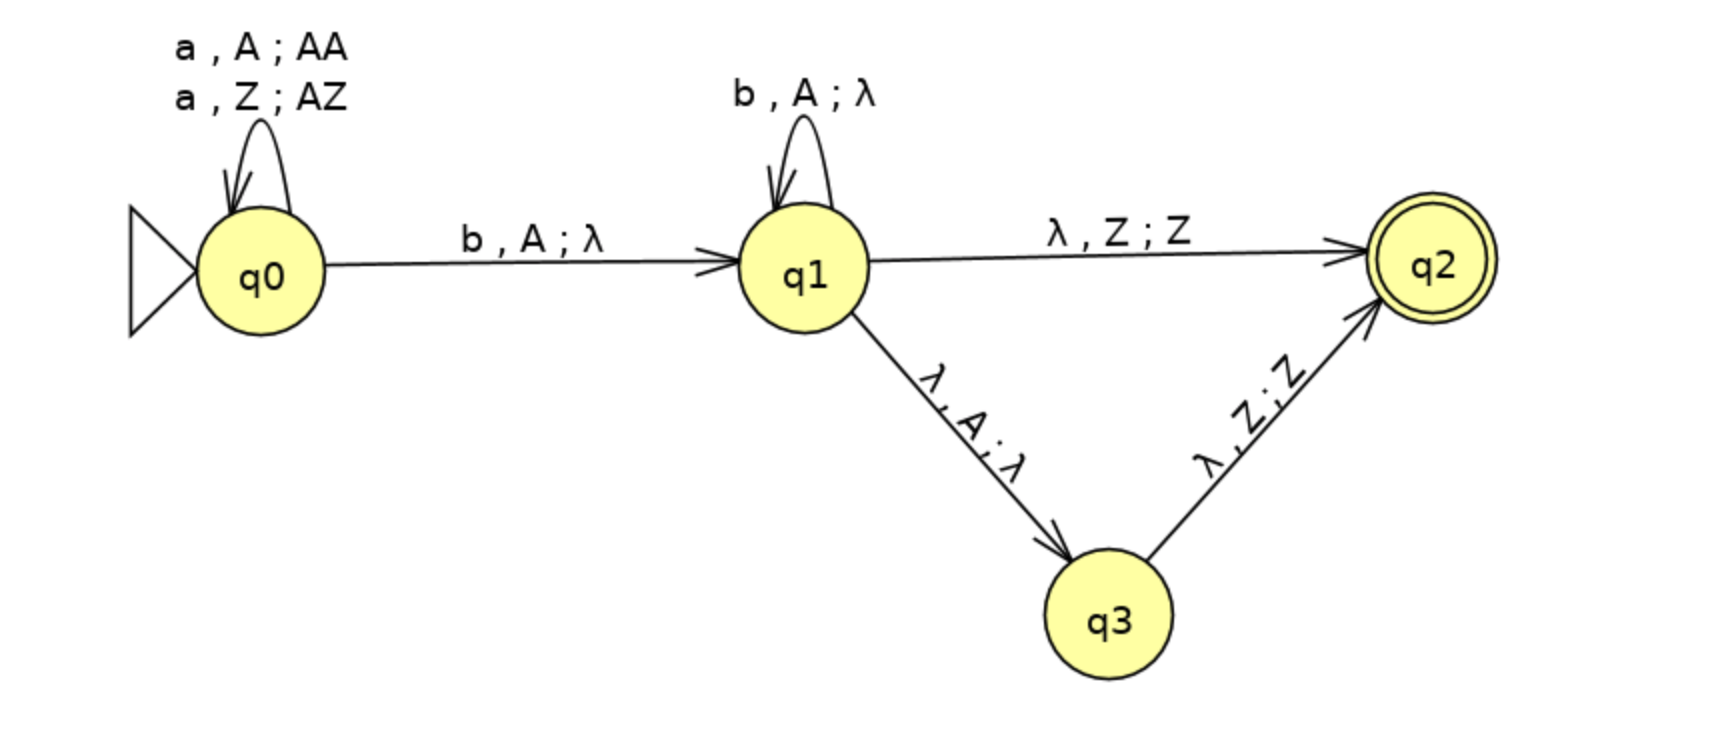
\includegraphics[scale=0.5]{Lez7sol6.png}
\end{enumerate}

\begin{comment}
       \item Sia data la CFG:\\
     \begin{minipage}{\linewidth}
        \centering $S \rightarrow aB$\\
        \centering $B \rightarrow Ab\ |\ b$\\
        \centering $A \rightarrow aB\ |\ a$\\
    \end{minipage}
    \\Dire: linguaggio accettato e definire un automa che accetti tale linguaggio.
\end{comment}
    % Bibliografia
    %\begin{thebibliography}{9}
        %  Alcune soluzio
    %\end{thebibliography}
    \end{document}